\section{Hyperchains design}
\graphicspath{ {./images/} }

The previous approaches had a lot to offer, but considering their weaknesses it
is worth thinking of some alternative solutions. PoW seems to work well only
with big computational effort being burned and PoS suffers from a huge amount of
security holes. The complicated algorithms required for plugging them usually
either do not solve the problem at all, moving it further to another layer of
abstraction or introducing extreme complexity on the protocol level.

Here we present a hybrid strategy that benefits from the stability of PoW
solutions but offers the scalability of PoS systems. A Hyperchain is a special
kind of blockchain that sticks to an already existing chain. They are going to
be called child and parent chain, respectively\cite{hyperchains}.

The parent chain can be almost any blockchain in the world. In general, we want
to use some big existing PoW based chains (at the time of writing, preferably
Bitcoin or Ethereum) to reuse their burned work to maintain the stability of the
child chain. We also propose a PoS–like election system to choose leaders on the
hyperchain. In this case, however, we employ a very reliable — and, most
importantly, unpredictable — source of randomness — the state of the parent
chain. The idea is not very new, though — some research into this topic exists
already\cite{blockchain_random}.

Having this machinery, it seems natural to start a new election each time a
(key)block has been mined on the parent chain. The next leader shall be chosen
depending on the hash of that block and selected with chances proportional to
their stake. The selection algorithm is abstract over this document — it is up
to the hyperchain to define the details.

\begin{figure}[b]
     \caption{Hyperchains interface}
     \centering
     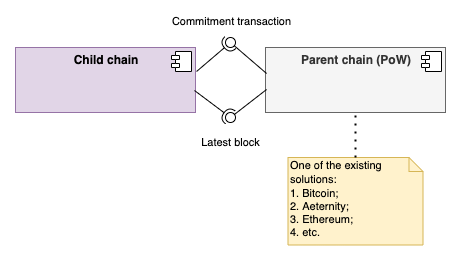
\includegraphics[scale=0.5]{hyperchains_interface}
\end{figure}

We define a group of leadership candidates called "delegates." Each delegate
needs to express their will of participation in the upcoming election by
publishing a commitment transaction onto the parent chain. It is important that
they clearly declare their view of the child chain and over which block they are
going to compete. Therefore, the commitment must consist of:

\begin{itemize}
\item The subject of delegation on the child chain
\item The block over which the delegate is going to build
\item Signature of the delegate from the child chain
\end{itemize}

One of the concepts key to the commitment idea is to be able to rely on the
parent chain's stability. We want to treat it as a rigid skeleton of the
hyperchain, which can be achieved by proper block hash linking. The elected
leader will be required to publish the key block on the child chain with a
cryptographic proof (referencing the parent) of their right to lead the upcoming
generation and publish micro blocks.

One dilemma that rises at this point is whether the commitment should reference
the latest key block, or the micro block of the child chain. Referencing a micro
block may seem more transparent, but we believe that it would lead to massive
forking (especially when some peers would not receive all of the blocks). One
must also consider the parent network's throughput. It may be impossible to fit
such a huge amount of commitments if we let delegates compete over each micro
block. The problem with referencing a key block is that the next leader could
steal the transactions and post them in their micro blocks. This, however, can
be resolved with a smarter feeing strategy. For instance, instead of giving the
full fee to the miner, we can split it up and give the bigger part to the next
leader who did include the previous leader's micro blocks in their continuation
of the history, as it happens in the BitcoinNG\cite{incentive_bcng}. Following
their election, the new leader posts a key block on the child chain, which
references the point on the parent, thus proving their right to lead the
generation. Besides that, they need to reference the micro block from the
previous generation, on which they want to mine.


\begin{figure}[h]
	\caption{Hyperchains Design}
	\centering
	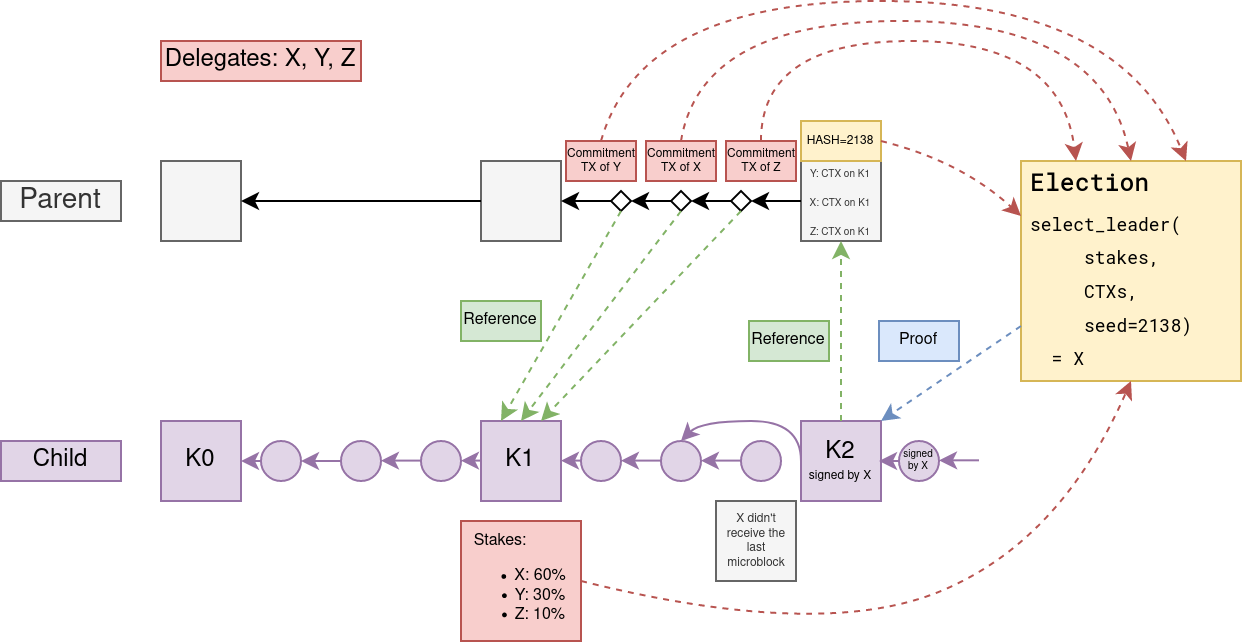
\includegraphics[scale=0.4]{hyperchains_design}
\end{figure}
